\documentclass[11 pt]{amsart}
\usepackage[top=1.00in,bottom=1.00in,left=1.00in,right=1.00in]{geometry}

\input{js_header.tex}

% Header from jtex file.
\usepackage{textcomp}
\graphicspath{{figs/}}
 

\hypersetup{
  colorlinks=true,linkcolor=blue,citecolor=blue,urlcolor=blue,
  pdftitle={TPRC -- Demographics}, pdfauthor={James Saxon}
  pdfpagemode={UseOutlines},
  bookmarksopen=true, bookmarksnumbered=true,
  pdfstartview={Fit}
}

\title[TPRC -- Demographics]{TPRC -- Demographics}
\date{\today}
\author[Saxon]{\vspace{-1.7em} James Saxon}
\email{jsaxon@uchicago.edu}
\address{Center for Data and Computing, University of Chicago \vspace{0.5em}}

\begin{document}




The coronavirus pandemic forced daily routines into the virtual spaces.
As both work and learning went remote, policymakers around the country
have sought to address ongoing inequities in Internet connectivity,
suddenly more acute than ever.
Data sources on Internet connectivity have substantial limitations
in measuring inequity.
In this Section, we highlight these limitations
while demonstrating what can nevertheless be done with the data.

In the American Community Survey (ACS)
the US Census Bureau asks respondents whether they have broadband Internet;
for the National Telecommunications and Information Administration (NTIA) supplement to the Current Population Survey (CPS),
they gather both data on connectitivity and online behaviors.
While the US Census Bureau is the "gold standard" of survey methodology,
the question of broadband access is coarse: the presence of a nominal, 25/3 Mbps contract.
Wealthy Americans have enjoyed higher bandwidths over time;
it is not possible to understand relative changes on the
\emph{intensive} margin (consumption or bandwidth) using the ACS or the CPS.
Unfortunately, subtlety is not required:
neighborhood economic indicators are strongly predictive of broadband contracts.
In Chicago for instance, the tract-level correlation between
log median household income and
the share of households with a broadband contract is 0.82,
as can be seen in Figure~\ref{fig:chicago_broadband_income}.
The CPS/NTIA data are not designed for use below the state-level,
but microdata allow breakdowns by race, ethnicity, and poverty status.\footnote{Nick: Let me know if this would be helpful, and I can get \href{https://github.com/JamesSaxon/neighborhood\_broadband/blob/master/census/ipums.ipynb}{these tables} into \LaTeX.}

\begin{figure}[]
\centering
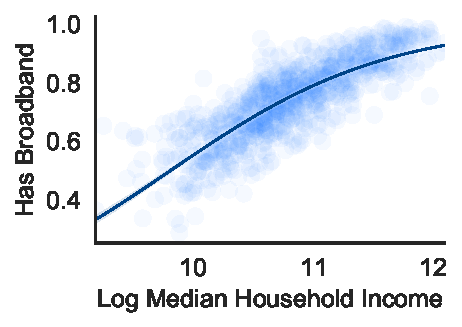
\includegraphics[width=0.45\textwidth]{broadband_income.pdf}
\caption{Census tract median household income versus share of households with broadband Internet, in Chicago.  A lowess curve is drawn. The linear correlation is 0.82. \label{fig:chciago_broadband_income}}
\end{figure}


Still, objective measures of real-world performance
could shed light on differences in online behaviors or
infrastructures by community.
For this purpose, we can examine data from SamKnows whiteboxes or
distributed measurements from Oookla speedtests, newly-released as Open Data.\cite{ookla}
The SamKnows data includes many measures of performance including bandwidth and consumption,
and the Ookla speedtest measures bandwidth and latency.
The challenge with these data is that they are highly non-representative.
The sampling frame for the SamKnows data was stratified by ISP and speed tier
(SamKnows worked with ISPs to under-represented speed cells),
rather than according to population demographics.\cite{samknows}
While no demographic indicators are provided,
block group or tract of residence is available for 94\% of the households included in the 2018 report.
If we aggregate block groups to the tracts that contain them,
we can compare tract median household income between SamKnows residences
to the American population (Figure~\ref{fig:rep_mhi}).
This reveals a significant offset:
a log diference of 0.13, implying incomes $14$\% higher in SamKnows ``neighborhoods."


A similar effect is apparent in the Ookla data.
The Ookla data are provided publicly as quad tiles (zoom level 16),
which are are roughly half a kilometer at the equator.
These do not map neatly to Census geographies,
but given the small tiles  we can allocate them approximately.
We assign each device from each quad tile in Chicago
to a random point within its tile;
we then merge these generated points to Census tracts.
This rough measure of the population of devices
can then be contrasted with the Census, by median household income, as above.
Just as for the SamKnows data, the devices are recorded in
neighborhoods that are markedly wealthier than the general population of Chicago.
The obvious reason for this is that the general population does not all have Internet.
However, if we weight Census populations by the share of households with Internet,
the gap remains significant.
This suggests that people in affluent areas are more likely to run speed tests,
even conditional on having Internet.
In short, both state-of-the-art
distributed measurements and official FCC samples
are systematically blind to vulnerable populations,
who do not run speedtests or volunteer for FCC measurements.

\begin{figure}[]
\centering
\subfloat[Ookla / Chicago]{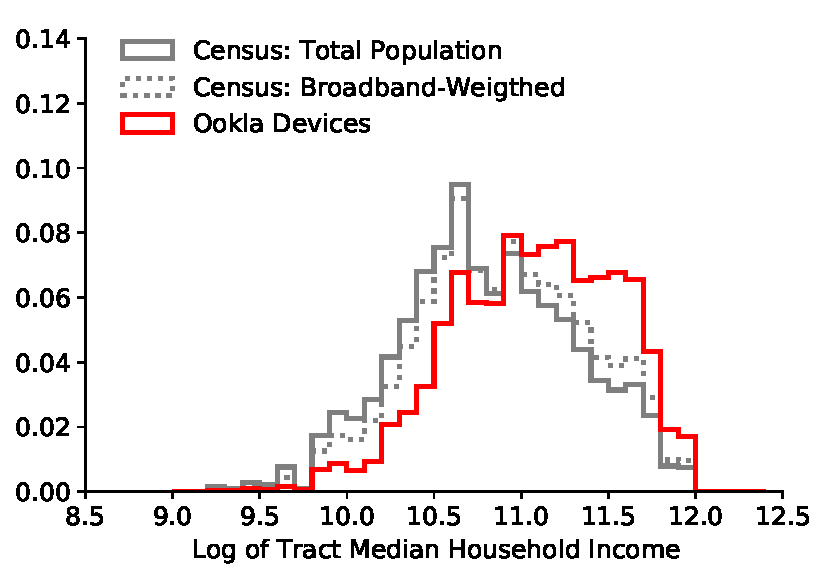
\includegraphics[width=0.47\textwidth]{rep_mhi_ookla_chicago.pdf}}
\subfloat[SamKnows / US]{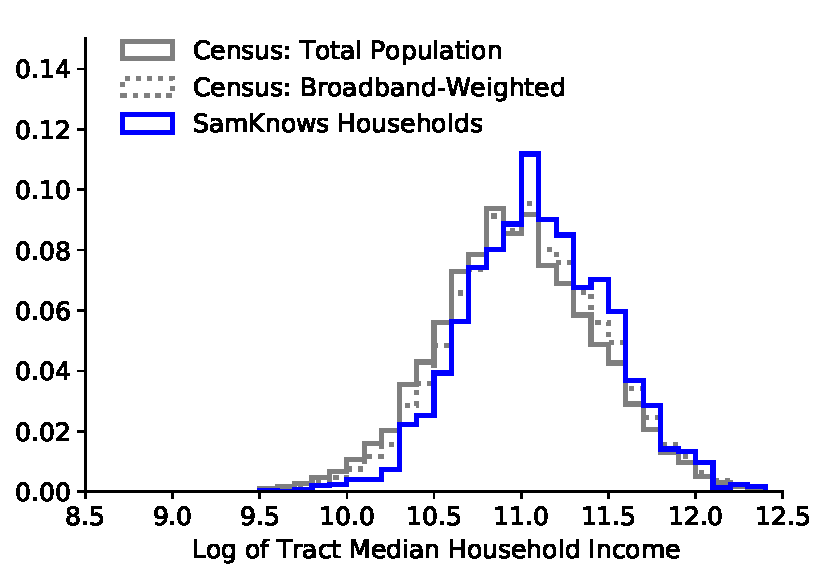
\includegraphics[width=0.47\textwidth]{rep_mhi_sk_us.pdf}}
\caption{Normalized distribution of Census tract median household income, weighted population counts, or for Ookla devices or SamKnows WhiteBox households.  The dotted lines weight Census populations by the share of neighborhood households with a broadband Internet contract. \label{fig:rep_mhi}}
\end{figure}


Though we emphasize the significant limitations of the data,
it \emph{is} possible to contrast performance over the course of the
coronavirus pandemic, by neighborhood,
for SamKnows households.
We first divide the SamKnows sample into three categories
by neighborhood income -- bottom quartile, middle quartiles, and highest quartile of the \emph{SamKnows sample}.
We then plot consumption and speed over time.
Within each income group,
we plot the 1st quartile, median, and 3rd quartile
of the distribution, from November 2019 until the most-recent release, August 2020.
These are shown in Figure~\ref{fig:sk_bandwidth}.
Conditional on \emph{having Internet},
households from wealthy neighborhoods do in fact purchase higher-bandwidth plans.
On the other hand, it is somewhat surprising to find in Figure~\ref{fig:sk_consumption}
from the perspective of consumption -- gigabytes per day --
households in lower income communities tend to use moderately \emph{more}
Internet, across the distribution (i.e., at all three quartiles).
These results remain somewhat inconclusive given the limitations of the data,
but they underscore the need for demographically-attuned
measurement of Internet performance and use.

\begin{figure}[]
\centering
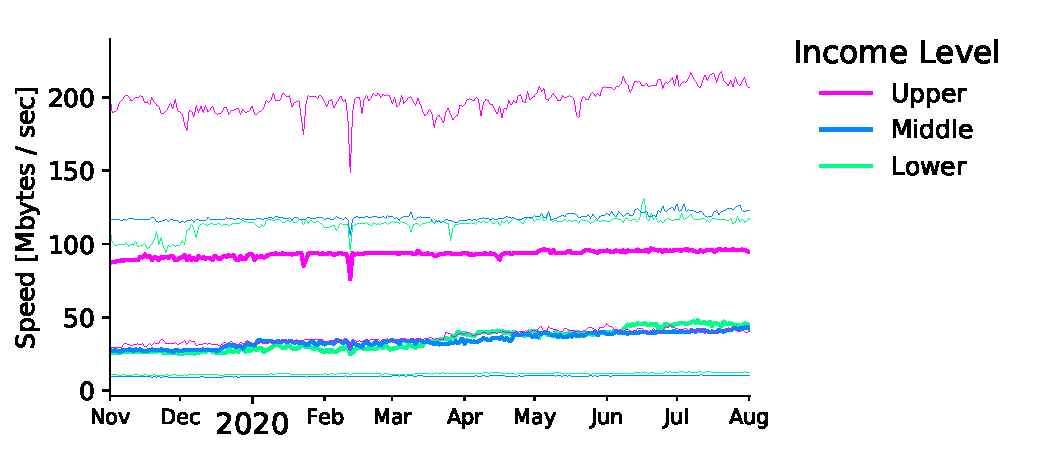
\includegraphics[width=0.7\textwidth]{sk_bandwidth.pdf}
\caption{Bandwidth measured by SamKnows data for low (first-quartile), medium (middle quartiles), and high-income tracts. Quartiles are of the SamKnows population. For each segment of the population the three lines show the first, second and third quartiles of bandwidth. \label{fig:sk_bandwidth}}
\end{figure}

\begin{figure}[]
\centering
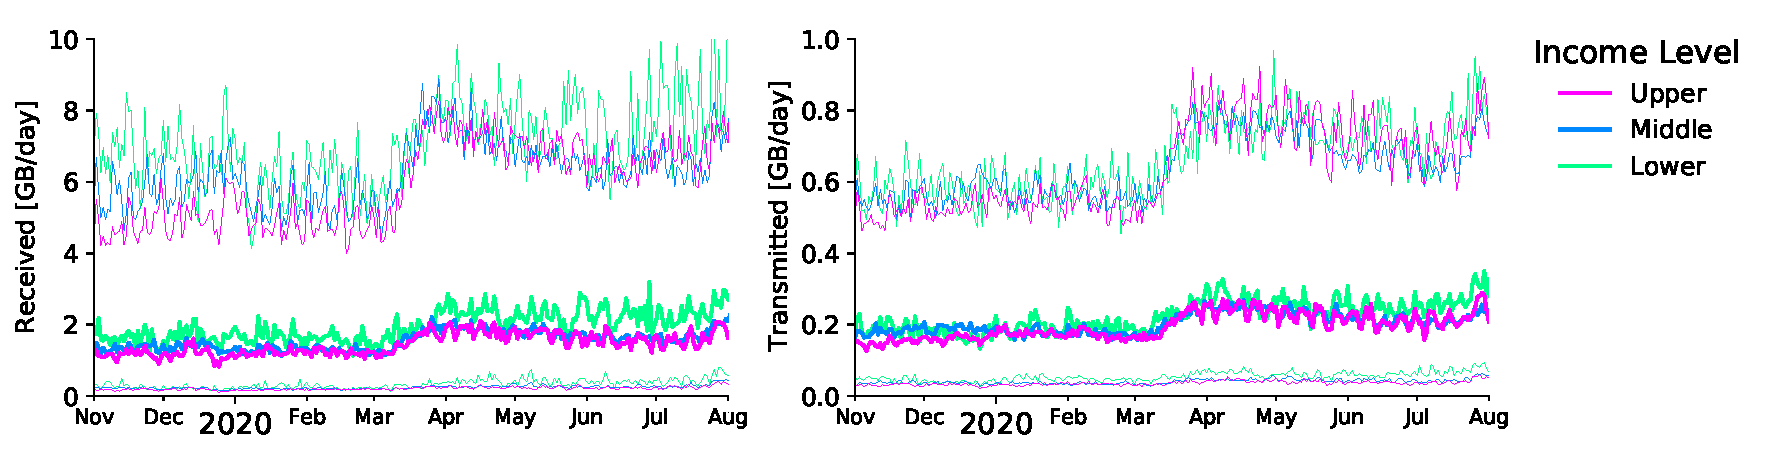
\includegraphics[width=1.0\textwidth]{sk_consumption.pdf}
\caption{Received and transmitted data, measured by SamKnows for low (first-quartile), medium (middle quartiles), and high-income tracts.  Quartiles are of the SamKnows population.  For each segment of the population the three lines show the first, second and third quartiles of consumption by day. \label{fig:sk_consumption}}
\end{figure}




\bibliographystyle{bibulous}
\bibliography{sources}



\end{document}

